\documentclass[a4paper, 12pt]{article}
\usepackage{titling}
\usepackage{array}
\usepackage{booktabs}
\usepackage{enumitem}
\usepackage{graphicx}
\setlength{\heavyrulewidth}{1.5pt}
\setlength{\abovetopsep}{4pt}
\graphicspath{{.}}

\usepackage[margin=1in]{geometry}

% Must be after geometry
\usepackage{fancyhdr}
\pagestyle{fancy}
\fancyhf{}
\rhead{AIR Homework 6}
\lhead{M. Nguyen, B. Ha \& E. Ovchinnikova}
\cfoot{\thepage}

\setlength{\droptitle}{-5em}

\title{Artificial Intelligence for Robots \\
				- Homework 6 -}
\author{Minh Nguyen, Bach Ha \& Evgenia Ovchinnikova}
\date{Lecture date: 10 November 2015}

\begin{document}

\maketitle

    \begin{enumerate}

    % Question 1
    \item Mind map for uninformed and informed search algorithms:
    
    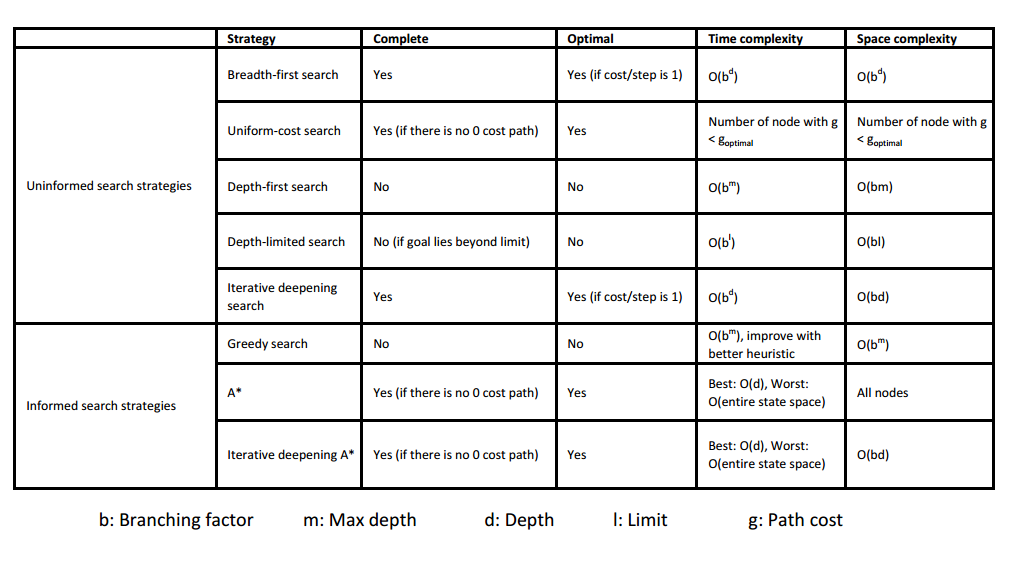
\includegraphics[scale=0.4]{Uninformedandinformedsearch.png} 
    
    % Question 2
    \item Explaination for statements:\vspace{0.5cm}\\
    \textbf{Statement}: Breadth-first search is a special case of uniform-cost search.\\
    \textbf{Explaination}: Uniform-cost search expand the node with the lowest path cost g(n). If all steps cost are equal, all nodes at the same depth would have the same g(n). Therefore Uniform-cost search would expand all nodes of a depth d before expanding nodes of depth d+1. This behaviour is the same behaviour of Breadth-first search.\\
	
	\textbf{Statement}: Breadth-first search, depth-first search, and uniform-cost search are special cases of Greedy Best-First Search\\
	\textbf{Explaination}:
	\begin{itemize}
		\item Breadth-first search: Greedy search function as BFS when the heuristic decrease consistently toward the goal and all steps costs are equal.
		\item Depth-first search: Greedy search function as DFS when the heuristic of nodes at depth d+1 are always smaller than the heuristic of nodes at depth d.
		\item Uniform-cost search: Greedy search function as Uniform-cost search when the heuristic decrease consistently toward the goal.
	\end{itemize}
	
	\vspace{0.5cm}
	\textbf{Statement}: Uniform-cost search is a special case of A* search\\
	\textbf{Explaination}: 
		\begin{itemize}
		\item Uniform-cost search: uses path cost g(n) to decide which node to expand.
		\item Uniform-cost search: uses value of f(n)= g(n) + h(n) to decide which node to expand.
		\end{itemize}
		It can easily be seen that, when all h(n) = 0, A* search would function as Uniform-cost search. 
		
	% Question 3
	\item A* search:
	\begin{itemize}
		\item A* is complete when there is no infinite path with finite cost.
		\item A* end the search process when the optimal goal is found.
		\item Behaviours of A* with a consistent heuristic: A* will expand the node with the lowest f(n) until the optimal goal with value of f($G_{optimal}$) is found. In case of a suboptimal goal with value of f($G_{sub}$) is found, A* would expand other nodes with value f(n) $<$ f($G_{sub}$).
	\end{itemize}
	
    \end{enumerate}

\end{document}
